\def\beginanswers{\iffalse}
%%\def\beginanswers{\iftrue}

\documentclass[10pt]{article}
\usepackage{amsmath,amsfonts,amsthm,amssymb}
\usepackage{graphicx}
\usepackage{enumerate}
\usepackage{upquote,textcomp}
\usepackage{listings}
\usepackage{color}

\definecolor{mygreen}{rgb}{0,0.6,0}
\definecolor{mygray}{rgb}{0.5,0.5,0.5}
\definecolor{mymauve}{rgb}{0.58,0,0.82}


\lstset{frame=tb,
  language=,
  aboveskip=3mm,
  belowskip=3mm,
  showstringspaces=false,
  columns=flexible,
  keepspaces=true,
  basicstyle={\small\ttfamily},
  numbers=none,
  numberstyle=\tiny\color{black},
  keywordstyle=\color{black},
  commentstyle=\color{black},
  stringstyle=\color{black},
  breaklines=true,
  breakatwhitespace=true,
  tabsize=3
}

\lstset{frame=tb,
  language=Python,
  aboveskip=3mm,
  belowskip=3mm,
  showstringspaces=false,
  columns=flexible,
  basicstyle={\small\ttfamily},
  numbers=none,
  numberstyle=\tiny\color{mygray},
  keywordstyle=\color{blue},
  commentstyle=\color{mygreen},
  stringstyle=\color{mymauve},
  breaklines=true,
  breakatwhitespace=true,
  tabsize=3
}


\newcommand{\vect}[1]{{\bf #1}}                 %for bold chars
\newcommand{\vecg}[1]{\mbox{\boldmath $ #1 $}}  %for bold greek chars
\newcommand{\matx}[1]{{\bf #1}}

\setlength{\parindent}{0in}
\setlength{\parskip}{1em}
\setlength{\textheight}{9.5in}
\setlength{\textwidth}{7in}
\setlength{\headsep}{0in}        % distance from top of page to address
\setlength{\topmargin}{-0.5in}
\setlength{\oddsidemargin}{-0.5in}
\setlength{\evensidemargin}{-0.5in}


\begin{document}
\thispagestyle{empty}

\vspace*{0.5in}

\begin{center}
\Large
\textbf{Open Source Software --- CSCI-4961 --- Summer 2019} \\
\textbf{Test 1} \\
\textbf{June 28, 2019}
\end{center}


%%%%%%%%%%%%%%%%%%%%%%%%%%%%%%%%%%%%%%%%%%%%%%%%%%%%%%%%%%%%%%%%%%%%%%%%
%%%%%%%%%%%%%%%%%%%%%%%%%%%%%%%%%%%%%%%%%%%%%%%%%%%%%%%%%%%%%%%%%%%%%%%%
\beginanswers
\begin{center}
\Large
\textbf{SOLUTIONS}
\end{center}

%%%%%%%%%%%%%%%%%%%%%%%%%%%%%%%%%%%%%%%%%%%%%%%%%%%%%%%%%%%%%%%%%%%%%%%%
\else
%%%%%%%%%%%%%%%%%%%%%%%%%%%%%%%%%%%%%%%%%%%%%%%%%%%%%%%%%%%%%%%%%%%%%%%%


\begin{center}

\textbf{\Large Name:} \underline {\hspace{2.0in}} \\

\bigskip
\bigskip

\centerline{
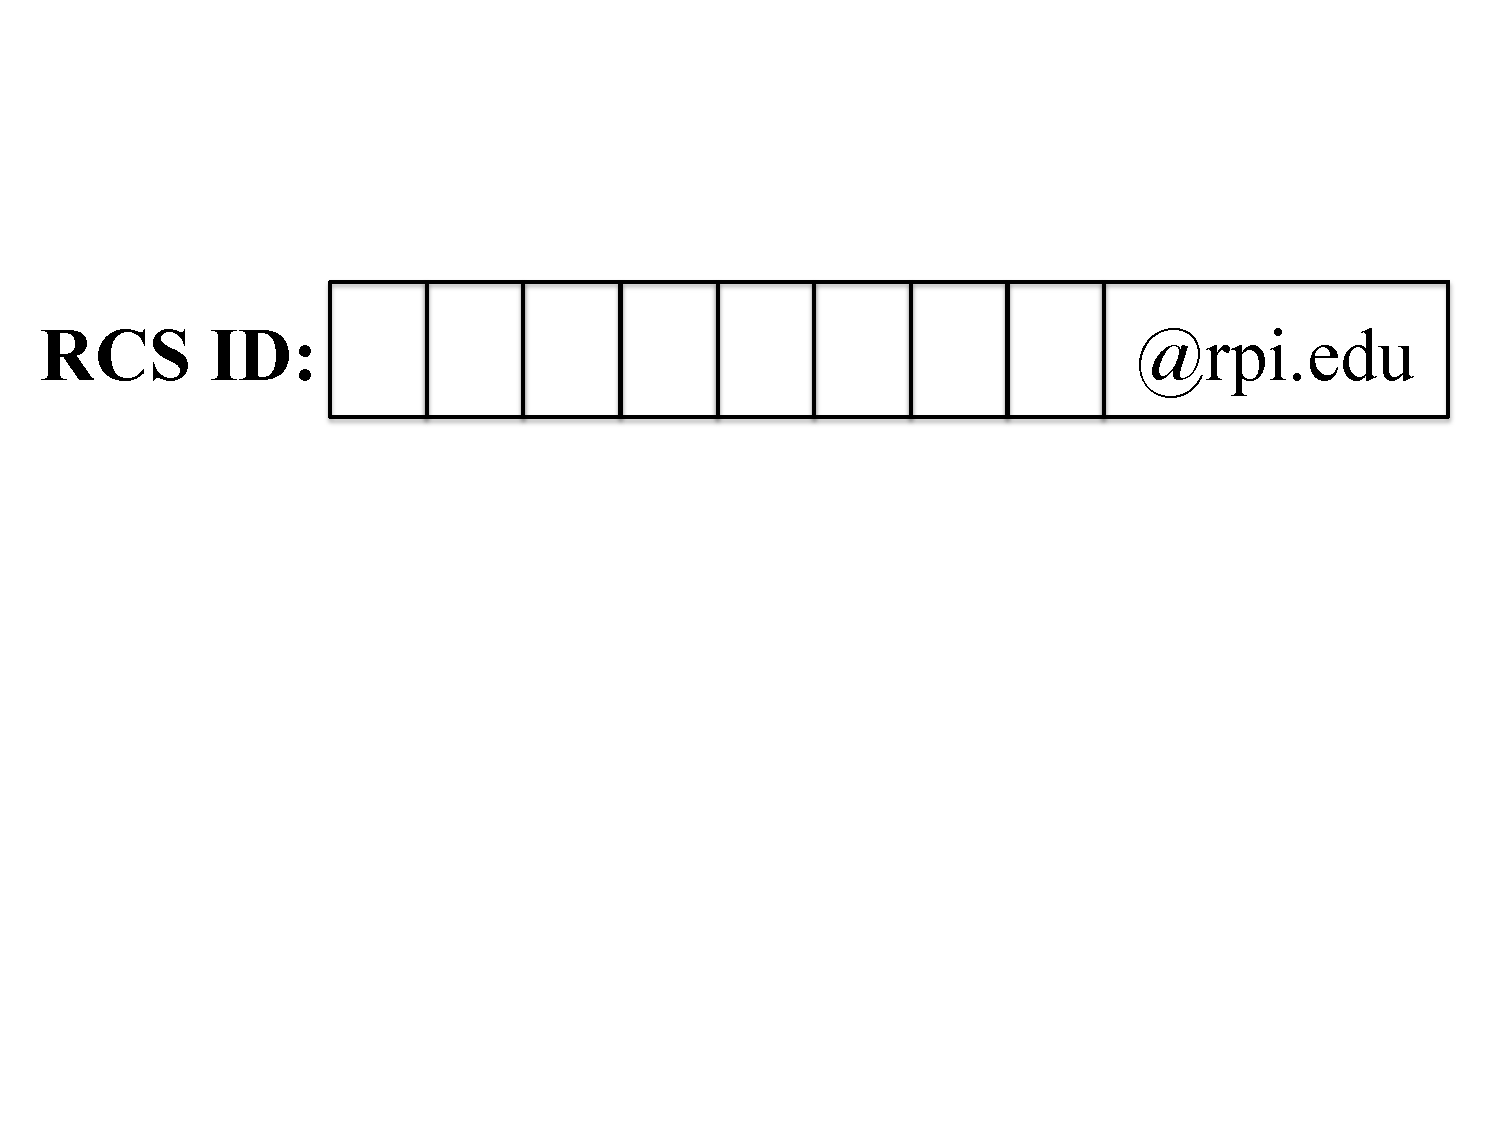
\includegraphics[height=0.5in]{boxes}
}

%%  \begin{tabular}{|p{0.1in}|p{0.1in}|p{0.1in}|p{0.1in}|p{0.1in}|p{0.1in}|p{0.1in}|p{0.1in}|l|}
%%    \hline \\
%%   & & & & & & & & \textbf{\large @rpi.edu} \\
%%  \hline
%%  \end{tabular} 
%%  
%%  \end{tabular}

\bigskip

\textbf{\Large RIN\#:} \underline {\hspace{1.5in}}  

\vspace*{0.4in}
{\large\bf Honor pledge: On my honor I have neither given
nor received aid on this exam.}

\vspace*{0.1in}
{\large\bf Please sign here to indicate that you agree with the honor pledge: \underline {\hspace{1.5in}}}
\end{center}

\vspace*{.45in} 

{\large\bf Instructions:}
\begin{itemize}
%%\item You have 90 minutes to complete this test.
\item Clearly print your name, RCS ID (in all caps.) and your RIN at the top of your exam.
\item This test is open book, open notes and open computer. You {\textbf may not} use the internet. Please turn off your wifi.
\item There are \textbf{7 questions} on this test worth a total of
  \textbf{100 points}.
\end{itemize}

\centering{\begin{tabular}{|c|c|r|}
	\hline
	Question & Score & Possible \\ \hline
	1 &  & 10 \\ \hline
	2 &  & 14 \\ \hline
	3 &  & 15 \\ \hline
	4 &  & 9 \\ \hline
	5 &  & 12 \\ \hline
	6 &  & 15 \\ \hline
	7 &  & 25 \\ \hline
	Total &  & 100 \\ \hline
\end{tabular}}

\newpage

%%%%%%%%%%%%%%%%%%%%%%%%%%%%%%%%%%%%%%%%%%%%%%%%%%%%%%%%%%%%%%%%%%%%%%%%
\fi
%%%%%%%%%%%%%%%%%%%%%%%%%%%%%%%%%%%%%%%%%%%%%%%%%%%%%%%%%%%%%%%%%%%%%%%%

\begin{enumerate}
	\item Answer the following short questions (10 pts)
	\begin{enumerate}
		\item Eric Raymond wrote, ``Before asking a technical question by e-mail, or in a newsgroup, or on a website chat board, do the following:'' and then listed 7 actions. List any 4 of them (4/10 pts)
		\begin{enumerate}[1]
			\beginanswers
			\item Try to find an answer by searching the archives of the forum or mailing list you plan to post to.
			\item Try to find an answer by searching the Web.
			\item Try to find an answer by reading the manual.
			\item Try to find an answer by reading a FAQ.
			\item Try to find an answer by inspection or experimentation.
			\item Try to find an answer by asking a skilled friend.
			\item If you're a programmer, try to find an answer by reading the source code.
			\else
			\item - 
			\bigskip
			\bigskip
			\bigskip
			\bigskip
			\item - 
			\bigskip
			\bigskip
			\bigskip
			\bigskip
			\item - 
			\bigskip
			\bigskip
			\bigskip
			\bigskip
			\item - 
			\bigskip
			\bigskip
			\bigskip
			\bigskip
			\fi
		\end{enumerate}	
	\item Name the RPI student who was sued by the RIAA for copyright infringement (1/10 pts)
	
	\beginanswers
	\bigskip
	Jesse Jordan
	(Aaron Sherman works as well, although Aaron was not mentioned in our reading.)
	\bigskip
	\else
	\begin{itemize}
		\bigskip
		\bigskip
		\item  - 
		\bigskip
		\bigskip
	\end{itemize}
	\fi
	\item Given the following regex expression \verb+^[a-zA-Z](.*)\.(html|jpg)$+, indicate \textbf{Match} if the string would be a match, or \textbf{No Match} if it would not. (5/10 pts)
	\beginanswers
		\begin{enumerate}[1]
		\bigskip
		\item test.html  \textbf{Match}
		\bigskip
		\bigskip
		\bigskip
		\item 2a38588hfquh.jpg  \textbf{No Match}
		\bigskip
		\bigskip
		\bigskip
		\item jpg.r  \textbf{No Match}
		\bigskip
		\bigskip
		\bigskip
		\item a@p239552u7894aghe.jpg  \textbf{Match}
		\bigskip
		\bigskip
		\bigskip
		\item htmljpg \textbf{No Match}
		\bigskip
		\bigskip
		\bigskip
		\end{enumerate}
	\else
		\begin{enumerate}[1]
		\bigskip
		\item test.html
		\bigskip
		\bigskip
		\bigskip
		\item 2a38588hfquh.jpg
		\bigskip
		\bigskip
		\bigskip
		\item jpg.r
		\bigskip
		\bigskip
		\bigskip
		\item a@p239552u7894aghe.jpg
		\bigskip
		\bigskip
		\bigskip
		\item htmljpg
		\bigskip
		\bigskip
		\bigskip
		\end{enumerate}
		\fi
	
	\end{enumerate}

 \newpage

	\item The diagram below represents a normal (non-open source) software procurement cycle. Fill in the diagram with the terms needed to complete it. (We know that 7 appears 2 times.)(14 pts)
	
	\begin{figure}[h]
		\centering
		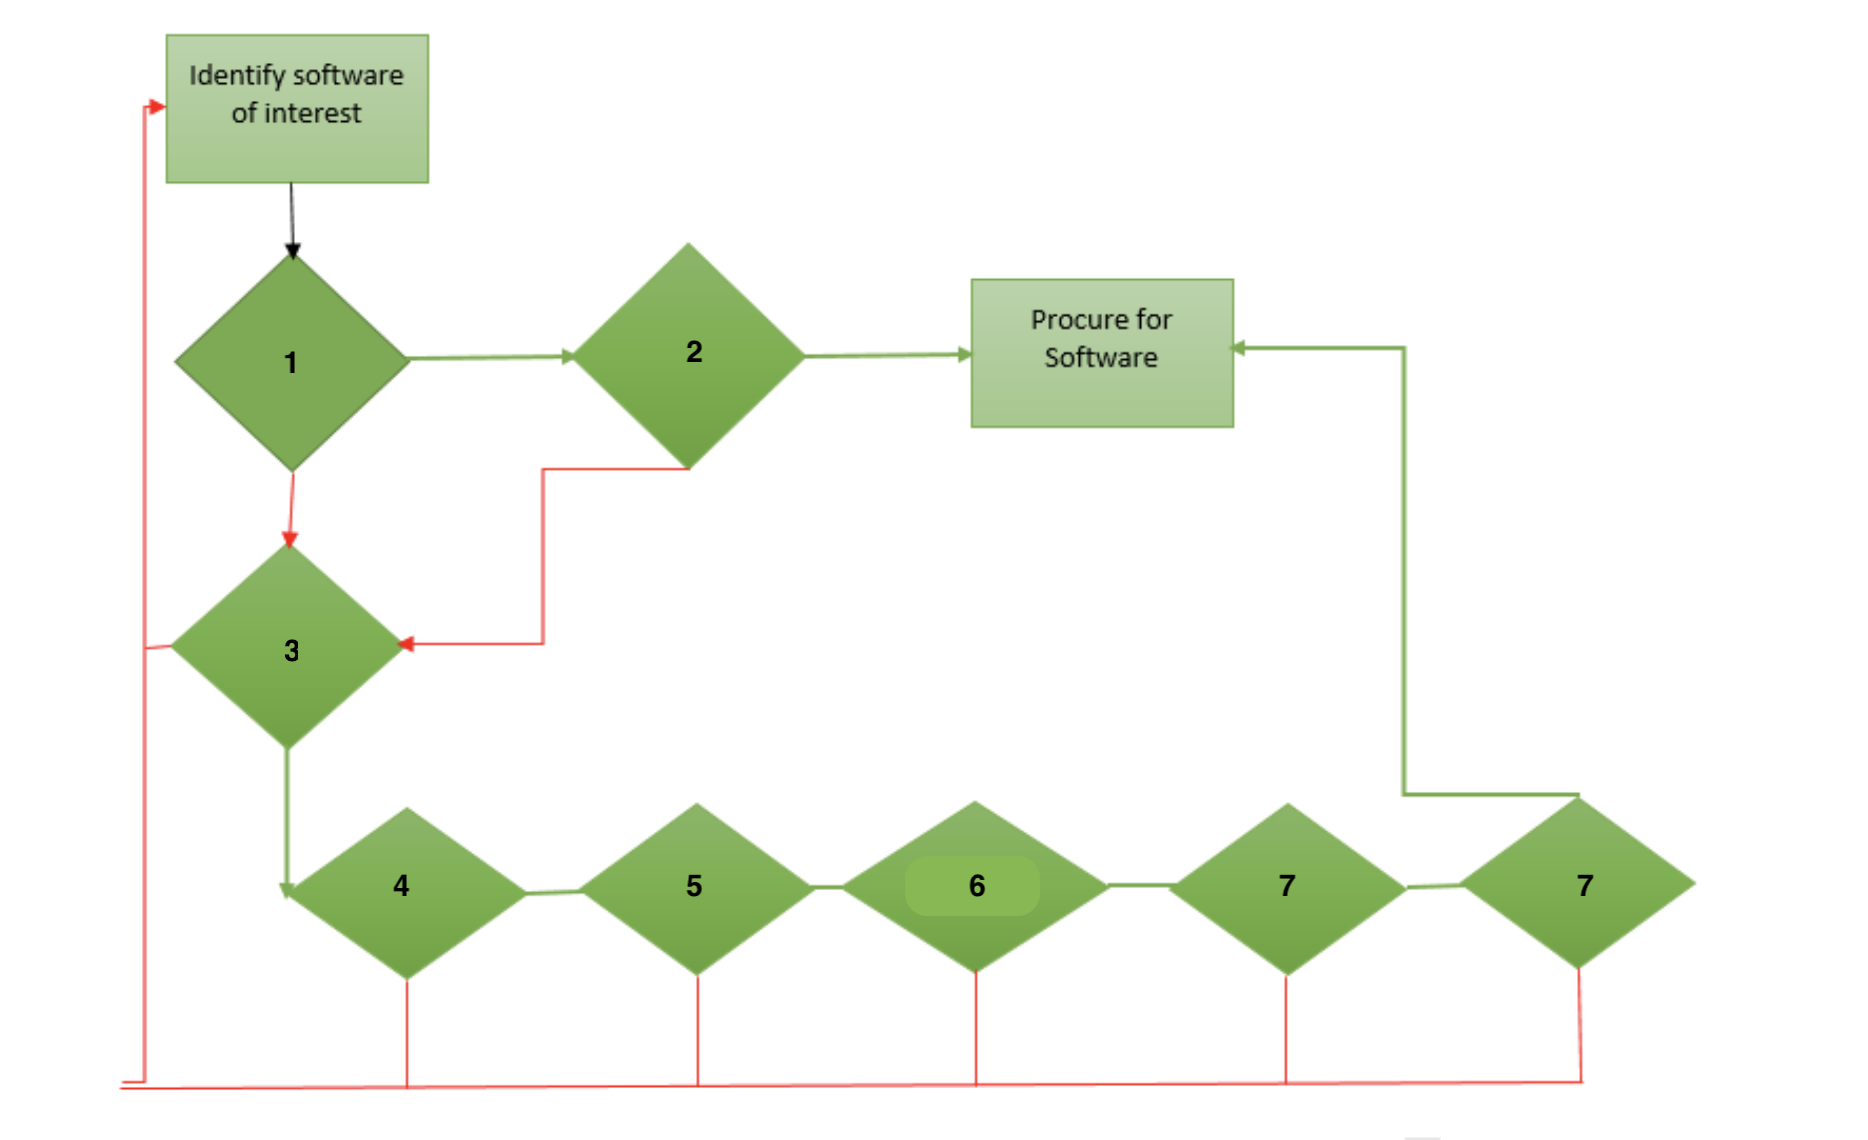
\includegraphics[width=.9\linewidth]{images/diag1.png}
		\label{fig:licensing}
	\end{figure}

\beginanswers
\begin{enumerate}[1]
	\item Is software for sale?
	\item Does standard license meet needs?
	\item Will vendor negotiate?
	\item Meet scope?
	\item Meet term?
	\item Renewal?
	\item Condition?
\end{enumerate}
\newpage
\else
\begin{enumerate}[1]
	\item -
	\bigskip
	\bigskip
	\bigskip
	\item -
	\bigskip
	\bigskip
	\bigskip
	\item -
	\bigskip
	\bigskip
	\bigskip
	\item -
	\bigskip
	\bigskip
	\bigskip
	\item -
	\bigskip
	\bigskip
	\bigskip
	\item -
	\bigskip
	\bigskip
	\bigskip
	\item -
	\bigskip
	\bigskip
	\bigskip
\end{enumerate}
\fi

	\item The Open Source Initiative defines 10 characteristics of open source software. For each of the following actions, indicate if the action is allowed or prohibited and the characteristic which allows or prohibits it. (15 pts)
	
	For example, for:
	
	\textit{Require a recipient of a derived work to contact the original author to get a license} the answer would be:
	
	\textbf{Prohibited, Distribution of License clause}
	
Each correct answer is worth 3 points with the \textbf{Allowed} or \textbf{Prohibited} worth 1 point and identifying the appropriate characteristic worth 2 points.

\beginanswers
\begin{enumerate}
		\item The author of a source code distribution allows the original code to be freely distributed requiring only attribution for the original authors and inclusion of the copyright notice, but requires that any derived works be distributed under an AGPL  license. (Original license is not AGPL)
	
	\textbf{Prohibited, Derived Works}
	\bigskip
		\item A user (recipient) gets a USB distribution of an open source family of products, all of the code on the USB is related and licensed simlarly. The user extracts one program from the USB and redistributes it as an independent program.
		
		\textbf{Allowed, License Must Not Be Specific to a Product}
		\bigskip
		\item An author requires that her source be maintained unchanged in any derivative works, but allows recipients to use \textit{git patch} files to implement and distribute modifications to the code.
		
		\textbf{Allowed, Integrity of the Author's Source Code}
		\bigskip
		\item An author distributes source under a BSD license, but adds a clause that prohibits the software from  being used by the military or by nuclear power plants.
		
		\textbf{Prohibited, No Discrimination Against Persons or Groups}
		\bigskip
		\item A user downloads the source code of several open source project from repositories on github onto a \$4.00 USB and then sells the offers the USB for sale on EBAY for \$10000 without paying or offering remuneration to the original author.

        \textbf{Allowed, Free Redistribution}
\bigskip
\end{enumerate}
\else
	\begin{enumerate}
	\item The author of a source code distribution allows the original code to be freely distributed, but requires that any derived works be distributed under an AGPL  license. (Original license is not AGPL)
	\bigskip
	\bigskip
	\bigskip
	\bigskip
	\bigskip
	\item A user (recipient) gets a USB distribution of an open source family of products, all of the code on the USB is related and licensed simlarly. The user extracts one program from the USB and redistributes it as an independent program.
	\bigskip
	\bigskip
	\bigskip
	\bigskip
	\bigskip
	\item An author requires that her source be maintained unchanged in any derivative works, but allows recipients to use \textit{git patch} files to implement and distribute modifications to the code.
	\bigskip
	\bigskip
	\bigskip
	\bigskip
	\bigskip
	\item An author distributes source under a BSD license, but adds a clause that prohibits the software from being used by the military or by nuclear power plants.
	\bigskip
	\bigskip
	\bigskip
	\bigskip
	\bigskip
	\item A user downloads the source code of several open source project from repositories on github onto a \$4.00 USB and then sells the offers the USB for sale on EBAY for \$10000 without paying or offering remuneration to the original author.
	\bigskip
	\bigskip
	\bigskip
	\bigskip
	\bigskip
\end{enumerate}
\fi
\newpage

\item Define the following types of intellectual property rights (9 pts):
\begin{enumerate}
\beginanswers
	\item Copyright
	\bigskip
Form of intellectual property, applicable to any expressed representation of a creative work, that grants the creator of an original work exclusive rights to its use and distribution, usually for a limited time.
	\bigskip
	\item Patent
	\bigskip
A set of exclusive rights granted by a sovereign state to an inventor or assignee for a limited period of time in
exchange for detailed public disclosure of an invention.
	\bigskip
	\item Trademark
	\bigskip
A recognizable sign, design, or expression which identifies products or services of a particular source from those of others.
	\bigskip
\else
	\item Copyright
	\bigskip
	\bigskip
	\bigskip
	\bigskip
	\bigskip
	\bigskip
	\bigskip
	\bigskip
	\item Patent
	\bigskip
	\bigskip
	\bigskip
	\bigskip
	\bigskip
	\bigskip
	\bigskip
	\bigskip
	\item Trademark
	\bigskip
	\bigskip
	\bigskip
	\bigskip
	\bigskip
	\bigskip
	\bigskip
	\bigskip
\fi
\end{enumerate}

\item Write LaTeX code to duplicate the document below. You can assume the photo  is ``images/pelican.jpg''. Your text should go on the next page. (12 pts):
\begin{figure}[h]
	\centering
	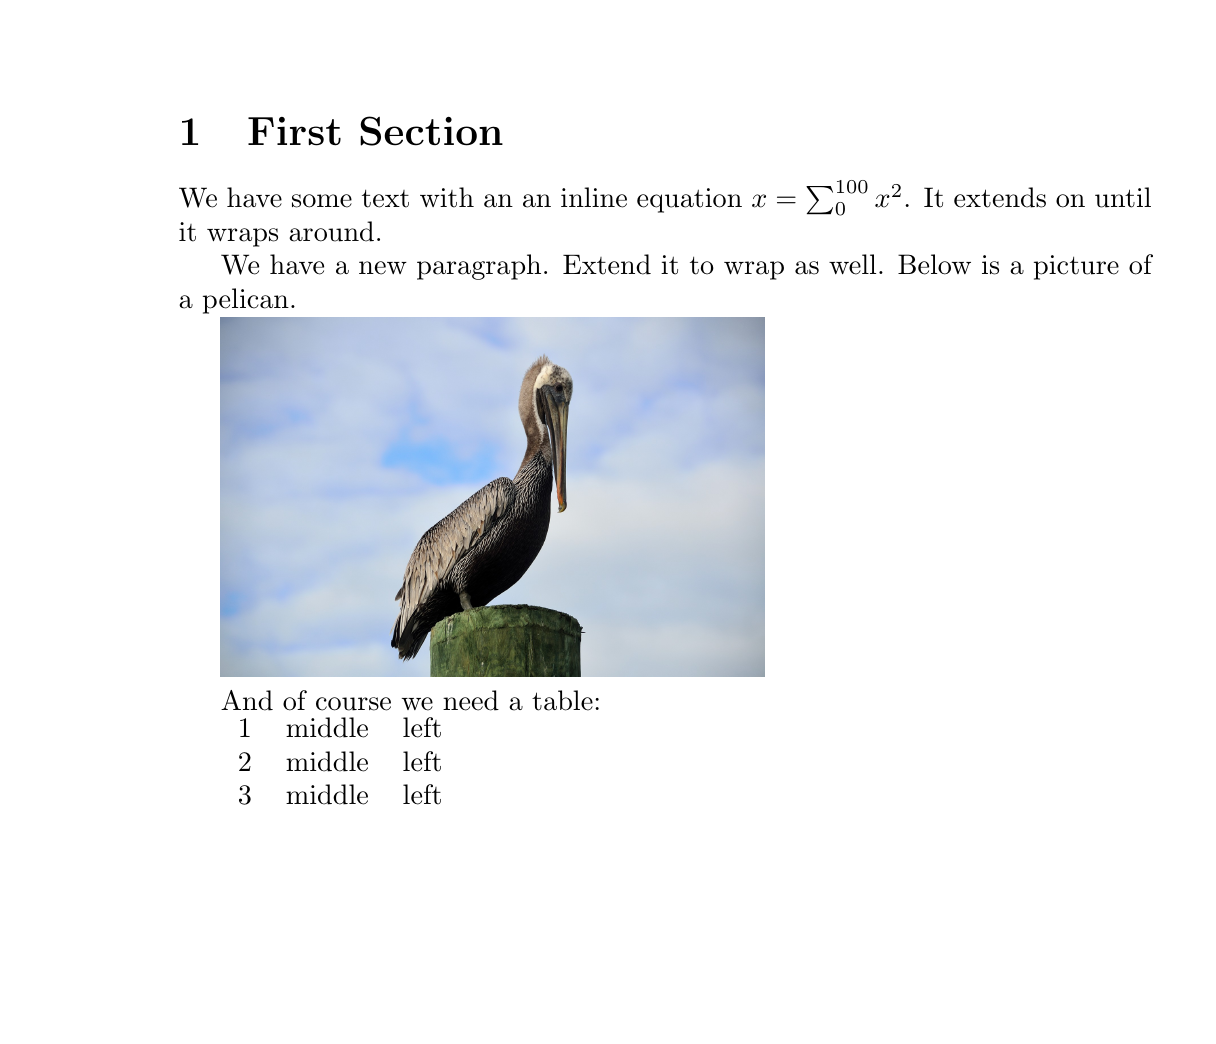
\includegraphics[width=0.6\linewidth]{images/test1.png}
\end{figure}

\newpage
\beginanswers

\begin{lstlisting}[language=tex]
\documentclass{article}
\usepackage[pdftex]{graphicx}
\begin{document}
\section{First Section}
We have some text with an an inline equation $x = \sum_0^{100} x^2$. It extends on until it wraps around.

We have a new paragraph. Extend it to wrap as well. Below is a picture of a pelican.

%scaling doesn't matter
\includegraphics[scale=0.10]{images/pelican.jpg} 

And of course we need a table:

\begin{tabular}{ccc}
1& middle	& left \\
2& middle & left \\
3 & middle & left \\
\end{tabular}

\end{document}
\end{lstlisting}
\else
Write your LaTeX in the box below (we gave you a start with some declarations):

\begin{lstlisting}[language=tex]
\documentclass{article}
\usepackage[pdftex]{graphicx}
\end{lstlisting}
\hspace*{-0.4in}\framebox(540,600){}
\fi

\newpage

\item Consider the following scenario. You are working in a ``blessed'' repository configuration. On your laptop you have a clone of your fork with two remotes set up. The remote \textbf{origin} points to your forked repository and \textbf{upstream} points to the blessed repositiory. 
All three repositories are out of synch. You can assume the blessed repository \textit{(upstream)} has:
\begin{itemize} \item a new file ``d.cxx'' \end{itemize} 
and your fork \textit{(origin)} has: 
\begin{itemize}
	\item a new file ``e.cxx''.
\end{itemize} 
Your local repository on your laptop has 
\begin{itemize}
	\item a new file named ``a.cxx'' and \item two modified  files ``b.cxx'' and ``c.cxx''.
\end{itemize} 
Your goal is to get all of these changes in the master branch in your fork \textit{(origin)} so you can make a pull request to the blessed repository. Give the sequence of git commands required to reach the state where all changes are present in your fork and you are ready for the pull request. (15 pts)

Write your git commands below

\beginanswers
\begin{lstlisting}
git add a.cxx
git add -u
git commit -m "Committing the local changes"
git pull origin master
git pull upstream master
git push origin master
\end{lstlisting}\else
\hspace*{-0.4in}\framebox(540,460){}
\fi
\newpage

\item Consider the ``Makefile'' shown below. 
\begin{lstlisting}[language=make]
m1: m1.o liba.a libb.so
	cc m1.o liba.a libb.so -o m1 -Wl,-rpath .
m2: m2.o libb.so
	cc m2.o libb.so -o m2 -Wl,-rpath .
m1.o: m1.c
	cc -c m1.c -o m1.o
m2.o: m2.c
	cc -c m2.c -o m2.o
libb.so: b.o
	cc -shared -o libb.so b.o
liba.a: a.o
	ar qc liba.a a.o
b.o: b.c
	cc -fPIC -c b.c -o b.o
a.o: a.c
	cc -c a.c -o a.o
m2.o: i.h
a.o: i.h
\end{lstlisting}
\begin{enumerate}
	\item Draw the dependency graph that depicts the Makefile below. Use dotted lines for implicit dependencies. (10 pts)	
	
	\beginanswers
	\begin{figure}[h]
	\centering
	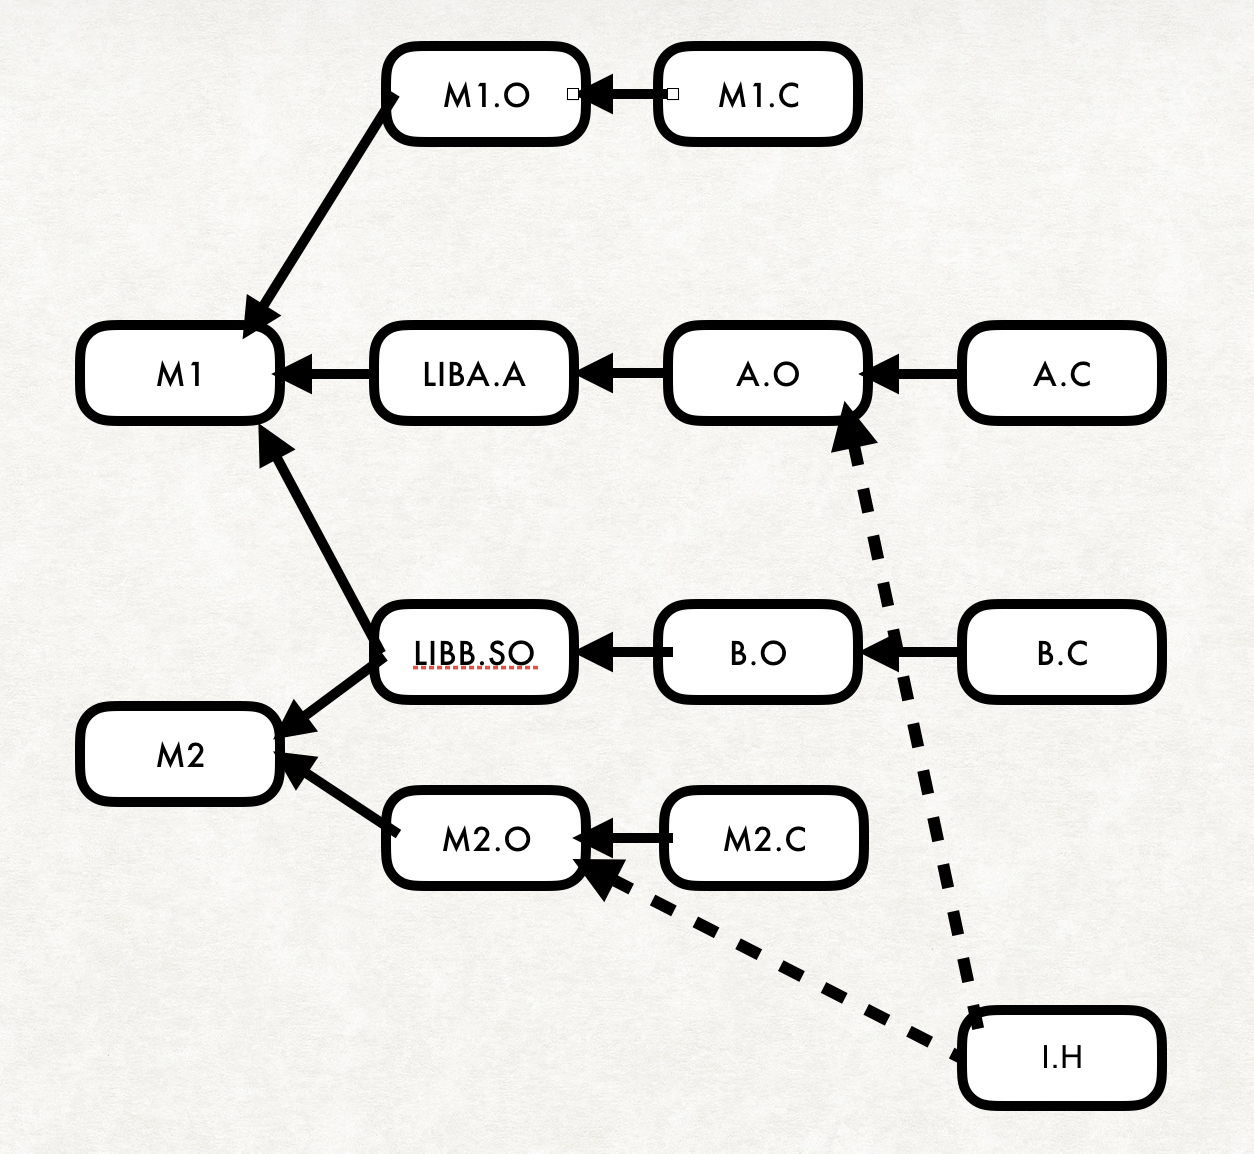
\includegraphics[width=.9\linewidth]{images/dependency.png}
	\label{fig:dependency}
\end{figure}

	\else
	\hspace*{-0.4in}\framebox(540,400){}
	\fi
	\newpage
	\item Makefiles should always have ``all'' and ``clean'' targets. Write the dependencies and commands for all and clean below (5pts):
	
		\beginanswers
\begin{lstlisting}[language=make]
all: m1 m2
clean:
	rm *.o *.so hi1 hi2
\end{lstlisting}
	\else
	\hspace*{-0.4in}\framebox(540,200){}
	\fi
	
	\item Now turn the Makefile into a CMakeLists.txt file. Add the commands to generate an install target to install ``m1'' and ``m2'' into ``bin'' and the shared library into ``lib'' (10 pts):
	
			\beginanswers
	\begin{lstlisting}[language=make]
	cmake_minimum_required(VERSION 3.0)
	project(Hello C)
	
	add_library(b SHARED b.c)
	add_library(a STATIC a.c i.h)
	
	add_executable(m1 m1.c)
	target_link_libraries(m1 a b)
	
	add_executable(m2 m2.c i.h)
	target_link_libraries(m2 b)
	
	install(TARGETS m1 DESTINATION bin)
	install(TARGETS m2 DESTINATION bin)
	install(TARGETS b DESTINATION lib)
	\end{lstlisting}
	\else
	\textbf{CMakeLists.txt}:
	
	\hspace*{-0.4in}\framebox(540,400){}
	\fi
	
\end{enumerate}
\end{enumerate}
\end{document}

